\subsection{Engine}
We divide the game loop into additional phases to avoid unnecessary coupling. We make it so that the phases only require the necessary data to be passed\dd, as opposed to passing the entire game. Figure \ref{fig:engine_flow} shows a full flow diagram of the engine, we briefly explain the different phases below:
\begin{itemize}
    \item Plan Move: Mark player objects as needing to be moved if the player has given a move command
    \item Apply Rules: Apply the rules as many times as possible
    \item Do Move: Move all objects marked as such, if there is an obstacle, see if we can move that obstacle
    \item Apply Late Rule: Apply the late rules as many times as possible.
    \item Check Victory: Check if we meet all the victory conditions, if not, do the loop again
\end{itemize}

The engine provides support to the game loop in the form of individual functions\dd. The game loop we design uses those function to run the game. We made this design decision to make it simple for other developers to create their own version of the loop by assembling the functions in a different order. Tool developers can also override the function to inject their changes without modifying the loop. For avoiding infinite loops, users can specify a limit on the number of times a rule can be applied.

\begin{figure}[!t]
    \centering
    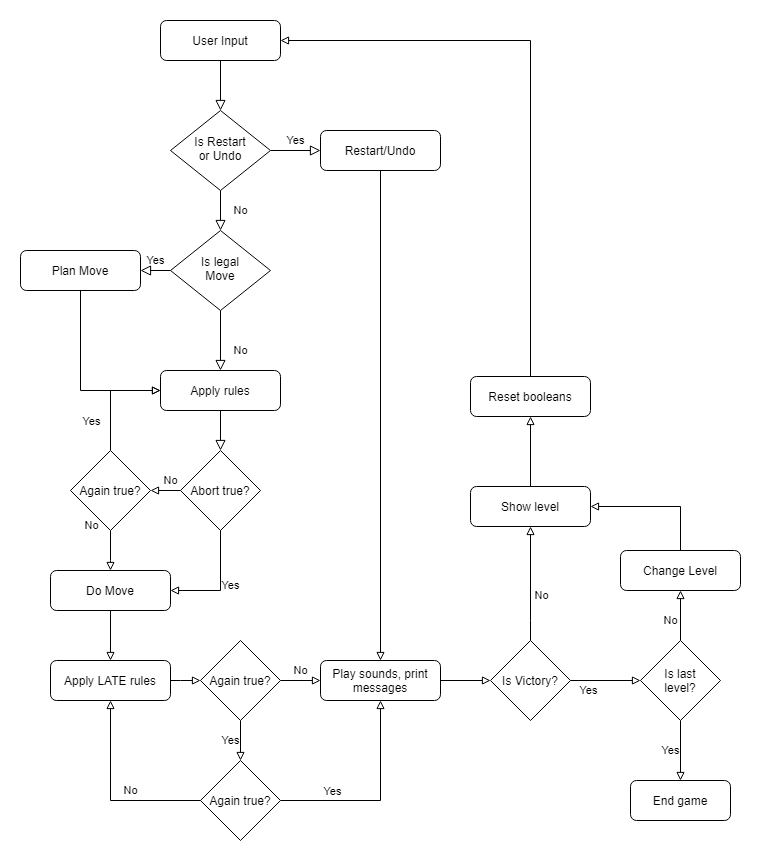
\includegraphics[width=1\textwidth]{images/Engine Flow.drawio.png}
    \caption{Engine flow graph}
    \label{fig:engine_flow}
\end{figure}

